\documentclass[11pt,a4paper,oneside]{report}
\usepackage{amsmath,amssymb,calc,ifthen}
\usepackage{float}
%\usepackage{cancel}
\usepackage[table,usenames,dvipsnames]{xcolor} % for coloured cells in tables
\usepackage{tikz}
% Allows us to click on links and references!
\usepackage{hyperref}
\usepackage{url}
\hypersetup{
colorlinks,
citecolor=black,
filecolor=black,
linkcolor=black,
urlcolor=black
}
% Nice package for plotting graphs
% See excellent guide:
% http://www.tug.org/TUGboat/tb31-1/tb97wright-pgfplots.pdf
\usetikzlibrary{plotmarks}
\usepackage{amsmath,graphicx}
\usepackage{epstopdf}
\usepackage{caption}
\usepackage{subcaption}
% highlight - useful for TODOs and similar
\usepackage{color}
\newcommand{\hilight}[1]{\colorbox{yellow}{#1}}
\newcommand\ci{\perp\!\!\!\perp} % perpendicular sign
\newcommand*\rfrac[2]{{}^{#1}\!/_{#2}} % diagonal fraction
\newcommand\SLASH{\char`\\}
\usepackage{listings}
% margin size
\usepackage[margin=1in]{geometry}
\tikzstyle{state}=[circle,thick,draw=black, align=center, minimum size=2.1cm,
inner sep=0]
\tikzstyle{vertex}=[circle,thick,draw=black]
\tikzstyle{terminal}=[rectangle,thick,draw=black]
\tikzstyle{edge} = [draw,thick]
\tikzstyle{lo} = [edge,dotted]
\tikzstyle{hi} = [edge]
\tikzstyle{trans} = [edge,->]
\definecolor{mygreen}{rgb}{0,0.6,0}
\definecolor{mygray}{rgb}{0.5,0.5,0.5}
\definecolor{mymauve}{rgb}{0.58,0,0.82}
\DeclareMathOperator*{\argmin}{arg\,min}
\DeclareMathOperator*{\argmax}{arg\,max}
\newcommand*{\Comb}[2]{{}^{#1}C_{#2}}
\lstset{ %
backgroundcolor=\color{white}, % choose the background color; you must add
%\usepackage{color} or \usepackage{xcolor}
basicstyle=\footnotesize, % the size of the fonts that are used for the
%code
breakatwhitespace=false, % sets if automatic breaks should only happen
%at whitespace
breaklines=true, % sets automatic line breaking
captionpos=b, % sets the caption-position to bottom
commentstyle=\color{mygreen}, % comment style
deletekeywords={...}, % if you want to delete keywords from the
%given language
escapeinside={\%*}{*)}, % if you want to add LaTeX within your code
extendedchars=true, % lets you use non-ASCII characters; for
%8-bits encodings only, does not work with UTF-8
frame=single, % adds a frame around the code
keepspaces=true, % keeps spaces in text, useful for keeping
%indentation of code (possibly needs columns=flexible)
keywordstyle=\color{blue}, % keyword style
language=Octave, % the language of the code
morekeywords={*,...}, % if you want to add more keywords to the set
numbers=left, % where to put the line-numbers; possible
%values are (none, left, right)
numbersep=5pt, % how far the line-numbers are from the code
numberstyle=\tiny\color{mygray}, % the style that is used for the line-numbers
rulecolor=\color{black}, % if not set, the frame-color may be changed
%on line-breaks within not-black text (e.g. comments (green here))
showspaces=false, % show spaces everywhere adding particular
%underscores; it overrides 'showstringspaces'
showstringspaces=false, % underline spaces within strings only
showtabs=false, % show tabs within strings adding particular
%underscores
stepnumber=2, % the step between two line-numbers. If it's
%1, each line will be numbered
stringstyle=\color{mymauve}, % string literal style
tabsize=2, % sets default tabsize to 2 spaces
title=\lstname % show the filename of files included with
%\lstinputlisting; also try caption instead of title
}
\title{Graphical Models Coursework 4}
\author{
Razvan Valentin Marinescu\\
Student Number: 14060166\\
\texttt{razvan.marinescu.14@ucl.ac.uk}
\and
Konstantinos Georgiadis\\
Student Number: 14110861\\
\texttt{konstantinos.georgiadis.14@ucl.ac.uk}
}
\begin{document}
\belowdisplayskip=12pt plus 3pt minus 9pt
\belowdisplayshortskip=7pt plus 3pt minus 4pt
\maketitle{}

\section*{Contributions}

Both of us solved all the problems on our own and compared the final answers. The solutions (apart from last question) were written in \LaTeX $\;$by Konstantinos with minor additions/brush-up by Razvan. 

\section*{Exercise 12.2}

\subsection*{1.}

We want to solve the following optimization problem:

$$w^\ast=\argmax_{w}p(y_{1:T}|\mathbf{x}_{1:T},\mathbf{w})$$

We rewrite the optimization problem in the following way:

\begin{align*}
\mathbf{w}^\ast&=\argmax_{w}p(y_{1:T}|\mathbf{x}_{1:T},\mathbf{w})\\
&=\argmax_{\mathbf{w}}\prod_{t=2}^T\frac{1}{\sqrt{2\pi}\sigma_t}e^{-\frac{(y_t-\mathbf{w}^\top\mathbf{x}_{t-1})^2}{2\sigma_t^2}}\\
&\text{The normalization denominators are constants which do not change the solution:}\\
&=\argmax_{\mathbf{w}}\prod_{t=2}^Te^{-\frac{(y_t-\mathbf{w}^\top\mathbf{x}_{t-1})^2}{2\sigma_t^2}}\\
&\text{We can also take the log of the function:}\\
&=\argmax_{\mathbf{w}}\log\left(\prod_{t=2}^Te^{-\frac{(y_t-\mathbf{w}^\top\mathbf{x}_{t-1})^2}{2\sigma_t^2}}\right)\\
&=\argmax_{\mathbf{w}}\log\left(e^{\sum_{t=2}^T-\frac{(y_t-\mathbf{w}^\top\mathbf{x}_{t-1})^2}{2\sigma_t^2}}\right)\\
&=\argmax_{\mathbf{w}}\sum_{t=2}^T-\frac{(y_t-\mathbf{w}^\top\mathbf{x}_{t-1})^2}{2\sigma_t^2}\\
&\text{We can remove the 1/2 factors and the minus signs by changing it into an argmin:}\\
&=\argmin_{\mathbf{w}}\sum_{t=2}^T\frac{(y_t-\mathbf{w}^\top\mathbf{x}_{t-1})^2}{\sigma_t^2}\\
&=\argmin_{\mathbf{w}}\sum_{t=2}^T\left(\frac{y_t}{\sigma_t}-\frac{\mathbf{w}^\top\mathbf{x}_{t-1}}{\sigma_t}\right)^2\\
&\text{We can rewrite this as a least squares problem as such:}\\
&=\argmin_{\mathbf{w}}||\mathbf{X}\mathbf{w}-\mathbf{y}||_2^2\text{, where: }\mathbf{X}=\left[ { \begin{array}{c} \mathbf{x}_1^\top/\sigma_2\\ ... \\ \mathbf{x}_{T-1}^\top/\sigma_T  \end{array} } \right], \mathbf{y}=\left[ { \begin{array}{c} y_2/\sigma_2\\ ... \\ y_{T}/\sigma_T  \end{array} } \right]\\
&\text{The common solution to which, is well known as the following:}\\
\mathbf{w}^\ast&=(\mathbf{X}^\top\mathbf{X})^{-1}\mathbf{X}^\top\mathbf{y}
\end{align*}

\subsection*{2.}

The hierarchical belief network is the following:

\begin{center}
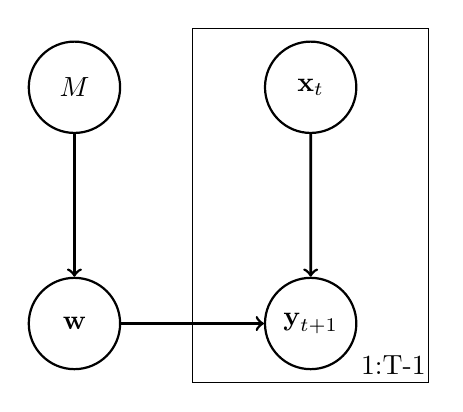
\begin{tikzpicture}[scale=1.5,auto,swap]

  \node[vertex,minimum size=33 pt] (m) at (-1,1) {$M$};      
  \node[vertex,minimum size=33 pt] (w) at (-1,-1) {$\textbf{w}$};   
  \node[vertex,minimum size=33 pt] (y) at (1,-1) {$\textbf{y}_{t+1}$};      
  \node[vertex,minimum size=33 pt] (x) at (1,1) {$\textbf{x}_t$}; 
  
%   % define the round nodes
%   \node[vertex,blue] (1a) at (-3.75877048314363,0) {$1$};
%   
%   \node[ellipse,draw, minimum size=25pt] (1a) at (-3,0) {$x_1,x_2,x_3$} ;
%   \node[rectangle,thick,draw=black] (2a) at (0,0) {$x_1,x_3$} ;
%   \node[ellipse,draw, minimum size=25pt] (3a) at (3,0) {$x_1,x_3,x_4$} ;


  
  %neighbouring graph
        
  \draw[->, line width=1]  (m)  -> (w);
  \draw[->, line width=1]  (w)  -> (y);
  \draw[->, line width=1]  (x)  -> (y);
  
  \draw (0,-1.5) -- (2,-1.5) -- (2,1.5) -- (0,1.5) -- (0,-1.5);
  \node at (1.7,-1.35) {1:T-1};  
 
\end{tikzpicture}
\end{center}
	
We initially start with equation 12.4.5:

$$p(M|\mathbf{x}_{1:T-1},\mathbf{y}_{2:T})=\frac{p(\mathbf{x}_{1:T-1},\mathbf{y}_{2:T}|M)p(M)}{p(\mathbf{x}_{1:T-1},\mathbf{y}_{2:T})}$$

The idea is to calculate the above probability for every different model M and then we will choose the one with the highest probability. Let us take for example two of them:

$$\frac{p(M=i|\mathbf{x}_{1:T-1},\mathbf{y}_{2:T})}{p(M=j|\mathbf{x}_{1:T-1},\mathbf{y}_{2:T})}=\frac{\frac{p(\mathbf{x}_{1:T-1},\mathbf{y}_{2:T}|M=i)p(M=i)}{p(\mathbf{x}_{1:T-1},\mathbf{y}_{2:T})}}{\frac{p(\mathbf{x}_{1:T-1},\mathbf{y}_{2:T}|M=j)p(M=j)}{p(\mathbf{x}_{1:T-1},\mathbf{y}_{2:T})}}=\frac{p(\mathbf{x}_{1:T-1},\mathbf{y}_{2:T}|M=i)p(M=i)}{p(\mathbf{x}_{1:T-1},\mathbf{y}_{2:T}|M=j)p(M=j)}$$

However, we are given that the prior p(M) is flat, therefore we need only:

$$\frac{p(M=i|\mathbf{x}_{1:T-1},\mathbf{y}_{2:T})}{p(M=j|\mathbf{x}_{1:T-1},\mathbf{y}_{2:T})}=\frac{p(\mathbf{x}_{1:T-1},\mathbf{y}_{2:T}|M=i)}{p(\mathbf{x}_{1:T-1},\mathbf{y}_{2:T}|M=j)}=\frac{\prod_{t=1}^{T-1}p(x_t)p(\mathbf{y}_{2:T}|\mathbf{x}_{1:T-1},M=i)}{\prod_{t=1}^{T-1}p(x_t)p(\mathbf{y}_{2:T}|\mathbf{x}_{1:T-1},M=j)}$$

By adjusting equation 12.4.6 we are now left with:

$$\frac{p(M=i|\mathbf{x}_{1:T-1},\mathbf{y}_{2:T})}{p(M=j|\mathbf{x}_{1:T-1},\mathbf{y}_{2:T})}=\frac{p(\mathbf{y}_{2:T}|\mathbf{x}_{1:T-1},M=i)}{p(\mathbf{y}_{2:T}|\mathbf{x}_{1:T-1},M=j)}=\frac{\int_{\mathbf{w}}p(\mathbf{w}|M=i) \prod_{t=1}^{T-1}p(\mathbf{y}_{t+1}|\mathbf{x}_t,\mathbf{w},M=i)}{\int_{\mathbf{w}}p(\mathbf{w}|M=j) \prod_{t=1}^{T-1}p(\mathbf{y}_{t+1}|\mathbf{x}_t,\mathbf{w},M=j)}$$

Since we are only interested in model comparison, we can equivalently use equation 12.4.7, after adjusting it to our current problem(we set $\alpha = 1$ right away and $\phi(x_t)=x_t$):

$$2\log p(\mathbf{y}_{2:T}|\mathbf{x}_{1:T-1},M=i)=-\left(\sum_{t=2}^{T}\log \left(2\pi\sigma_t^2\right)+\frac{y_t^2}{\sigma_t^2}\right)+\mathbf{b}^\top\mathbf{A}^{-1}\mathbf{b}-\log \det (\mathbf{A})$$

where:

$$\mathbf{A}=\mathbf{I}+\sum_{t=1}^{T-1}\frac{1}{\sigma_{t+1}^2}\mathbf{x}_t\mathbf{x}_t^\top, \mathbf{b}=\sum_{t=1}^{T-1}\frac{1}{\sigma_{t+1}^2}y_{t+1}\mathbf{x}_t$$

We also note that the first term is not affected by the model choice and therefore is not required in the computation. Therefore, we only need to calculate for each model the following and then find the maximum value:

$$\mathbf{b}^\top\mathbf{A}^{-1}\mathbf{b}-\log \det (\mathbf{A})$$

\subsection*{3.}

The MATLAB code used:

\begin{lstlisting}
clear all; clc; close all;
import brml.*
load('dodder.mat');
ModelLikelihoods = zeros(2^6-1,1);
for M = 1:2^6-1
    binary = logical(de2bi(M,6));
    A = eye(sum(binary));
    b = zeros(sum(binary),1);
    for t = 1:T-1
        A = A + (x(binary,t)*x(binary,t)')/(sigma(t+1)^2);
        b = b + (y(t+1)*x(binary,t))/(sigma(t+1)^2);
        %ModelLikelihoods(M) = ModelLikelihoods(M) + log(2*pi*sigma(t)^2) + (y(t)^2)/(sigma(t)^2);
    end
    ModelLikelihoods(M) = - ModelLikelihoods(M) + b'*(A\b)-log(det(A));
end
[~,BestModel] = max(ModelLikelihoods);
de2bi(BestModel,6)
\end{lstlisting}

MATLAB prints out that the best model is the one using only the first four variables:

ans =

     1     1     1     1     0     0

\section*{Exercise 12.3}

\subsection*{1.}
We want to show that:

\begin{align*}\frac{1}{(2\pi \alpha^{-1})^{K/2}}e^{-\frac{\alpha}{2}\mathbf{w}^\top \mathbf{w}}\frac{1}{(2\pi \sigma^{2})^{N/2}}e^{-\frac{1}{2\sigma^2}\sum_n (y^n-\mathbf{w}^\top \phi(x^n))^2} =
\frac{1}{(2\pi \alpha^{-1})^{K/2}}\frac{1}{(2\pi \sigma^{2})^{N/2}}e^{-\frac{1}{2\sigma^2}\sum_n(y^n)^2}e^{-\frac{1}{2}\mathbf{w}^\top\mathbf{A}\mathbf{w}+\mathbf{b}^\top\mathbf{w}}
\end{align*}

We prove this using the following equivalences:


\fontsize{11pt}{11pt}\selectfont
\hspace*{-2cm}\vbox{\begin{align*}
\text{Removing the fractions:}&\\
e^{-\frac{\alpha}{2}\mathbf{w}^\top \mathbf{w}}e^{-\frac{1}{2\sigma^2}\sum_n (y^n-\mathbf{w}^\top \phi(x^n))^2}&=e^{-\frac{1}{2\sigma^2}\sum_n(y^n)^2}e^{-\frac{1}{2}\mathbf{w}^\top\mathbf{A}\mathbf{w}+\mathbf{b}^\top\mathbf{w}}\\
\text{Taking the logarithm:}&\\
-\frac{\alpha}{2}\mathbf{w}^\top \mathbf{w}-\frac{1}{2\sigma^2}\sum_n (y^n-\mathbf{w}^\top \phi(x^n))^2&=-\frac{1}{2\sigma^2}\sum_n(y^n)^2-\frac{1}{2}\mathbf{w}^\top\mathbf{A}\mathbf{w}+\mathbf{b}^\top\mathbf{w}\\
\text{Expanding the quadratic:}&\\
-\frac{\alpha}{2}\mathbf{w}^\top \mathbf{w}-\frac{1}{2\sigma^2}\left(\sum_n (y^n)^2-2y^n\mathbf{w}^\top\phi(x^n)+(\mathbf{w}^\top\phi(x^n))^2\right)&=-\frac{1}{2\sigma^2}\sum_n(y^n)^2-\frac{1}{2}\mathbf{w}^\top\mathbf{A}\mathbf{w}+\mathbf{b}^\top\mathbf{w}\\
\text{Distributing the sum and rearranging:}&\\
-\frac{\alpha}{2}\mathbf{w}^\top \mathbf{w}-\frac{1}{2\sigma^2}\sum_n (y^n)^2+\frac{1}{\sigma^2}\sum_ny^n\mathbf{w}^\top\phi(x^n)-\frac{1}{2\sigma^2}\sum_n(\mathbf{w}^\top\phi(x^n)\mathbf{w}^\top\phi(x^n))&=-\frac{1}{2\sigma^2}\sum_n(y^n)^2-\frac{1}{2}\mathbf{w}^\top\mathbf{A}\mathbf{w}+\mathbf{b}^\top\mathbf{w}\\
\text{Removing the sum over y's and rearranging:}&\\
-\frac{\alpha}{2}\mathbf{w}^\top \mathbf{I} \mathbf{w}+\mathbf{w}^\top\frac{1}{\sigma^2}\sum_ny^n\phi(x^n)-\mathbf{w}^\top\frac{1}{2\sigma^2}\sum_n(\phi(x^n)\phi(x^n)^\top)\mathbf{w}&=-\frac{1}{2}\mathbf{w}^\top\mathbf{A}\mathbf{w}+\mathbf{b}^\top\mathbf{w}\\
\text{Substituting with the definition of b and rearranging:}&\\
-\frac{1}{2}\mathbf{w}^\top\left(\alpha \mathbf{I} + \frac{1}{\sigma^2}\sum_n\phi(x^n)\phi(x^n)^\top \right) \mathbf{w}+\mathbf{w}^\top\mathbf{b}&=-\frac{1}{2}\mathbf{w}^\top\mathbf{A}\mathbf{w}+\mathbf{b}^\top\mathbf{w}\\
\text{Substituting with the definition of A and rearranging:}&\\
-\frac{1}{2}\mathbf{w}^\top\mathbf{A} \mathbf{w}+\mathbf{w}^\top\mathbf{b}&=-\frac{1}{2}\mathbf{w}^\top\mathbf{A}\mathbf{w}+\mathbf{w}^\top\mathbf{b}\\
\end{align*}}

\subsection*{2.}
We now want to find out the expression for $2\log p(y^1,...,y^N|x^1,...,x^N,K)$:
\fontsize{12pt}{12pt}\selectfont
\begin{align*}
2\log p(y^1,...,y^N|x^1,...,x^N,K)&=\\
2\log\left( \int_{\mathbf{w}} \frac{1}{(2\pi \alpha^{-1})^{K/2}}\frac{1}{(2\pi \sigma^{2})^{N/2}}e^{-\frac{1}{2\sigma^2}\sum_n(y^n)^2}e^{-\frac{1}{2}\mathbf{w}^\top\mathbf{A}\mathbf{w}+\mathbf{b}^\top\mathbf{w}}  d\mathbf{w} \right)&=\\
2\log\left( \frac{1}{(2\pi \alpha^{-1})^{K/2}}\frac{1}{(2\pi \sigma^{2})^{N/2}}e^{-\frac{1}{2\sigma^2}\sum_n(y^n)^2} \int_{\mathbf{w}} e^{-\frac{1}{2}\mathbf{w}^\top\mathbf{A}\mathbf{w}+\mathbf{b}^\top\mathbf{w}}  d\mathbf{w} \right)&=\\
\text{Based on 8.4.13}:&\\
2\log\left( \frac{1}{(2\pi \alpha^{-1})^{K/2}}\frac{1}{(2\pi \sigma^{2})^{N/2}}e^{-\frac{1}{2\sigma^2}\sum_n(y^n)^2} \sqrt{\det(2\pi\mathbf{A}^{-1})}e^{\frac{1}{2}\mathbf{b}^\top\mathbf{A}^{-1}\mathbf{b}} \right)&=\\
2\left( -\log (2\pi \alpha^{-1})^{K/2} -\log (2\pi \sigma^{2})^{N/2} -\frac{1}{2\sigma^2}\sum_n(y^n)^2 + \log(\sqrt{\det(2\pi\mathbf{A}^{-1})}) + \frac{1}{2}\mathbf{b}^\top\mathbf{A}^{-1}\mathbf{b} \right)&=\\
2\left( -\frac{K}{2}\log (2\pi \alpha^{-1}) -\frac{N}{2}\log (2\pi \sigma^{2}) -\frac{1}{2\sigma^2}\sum_n(y^n)^2 + \log(\sqrt{(2\pi)^K\det(\mathbf{A}^{-1})}) + \frac{1}{2}\mathbf{b}^\top\mathbf{A}^{-1}\mathbf{b} \right)&=\\
-K\log (2\pi \alpha^{-1}) -N\log (2\pi \sigma^{2}) -\frac{1}{\sigma^2}\sum_n(y^n)^2 + \log((2\pi)^K\det(\mathbf{A})^{-1}) + \mathbf{b}^\top\mathbf{A}^{-1}\mathbf{b} &=\\
-K\log (2\pi) -K\log(\alpha^{-1}) -N\log (2\pi \sigma^{2}) -\frac{1}{\sigma^2}\sum_n(y^n)^2 + K\log(2\pi)+\log(\det(\mathbf{A})^{-1}) + \mathbf{b}^\top\mathbf{A}^{-1}\mathbf{b} &=\\
K\log(\alpha) -N\log (2\pi \sigma^{2}) -\frac{1}{\sigma^2}\sum_n(y^n)^2 -\log(\det(\mathbf{A})) + \mathbf{b}^\top\mathbf{A}^{-1}\mathbf{b} &\\
\end{align*}

\subsection*{3.}

We didn't understand what we were meant to do for this point.

\section*{Exercise 23.4}

Here we only made two changes to the code. We changed the input string variable s and also at the end, when the most likely set of words (that are in the dictionary) are found, we make MATLAB output the log likelihood:
    if val; \\
        disp([num2str(t) ':' str]);\\
        log(maxval.table{t}) \\
    end\\\\
    
    MATLAB outputs for the most likely state:\\\\\
    659:the monkey is on the branch\\

And the log likelihood of that state is:\\\\\

  -94.5250


\begin{lstlisting}
clear all; clc; close all;
import brml.*;
load freq; % http://www.data-compression.com/english.shtml
l = {'a','b','c','d','e','f','g','h','i','j','k','l','m','n','o','p','q','r','s','t','u','v','w','x','y','z',' '};
load typing; % get the A transition and B emission matrices
figure(1); imagesc(A); set(gca,'xtick',1:27); set(gca,'xticklabel',l); set(gca,'ytick',1:27); set(gca,'yticklabel',l)
colorbar; colormap hot; title('transition')
figure(2); imagesc(B); set(gca,'xtick',1:27); set(gca,'xticklabel',l); set(gca,'ytick',1:27); set(gca,'yticklabel',l)
colorbar; colormap hot; title('emission')
ph1=condp(ones(27,1)); % uniform first hidden state distribution

%s = 'kezrninh'; Nmax=200; % observed sequence
s = 'rgenmonleunosbpnntje vrancg';  Nmax=1200; % observed sequence (brilliant is the answer)
v=double(s)-96; v=replace(v,-64,27); % convert to numbers

% find the most likely hidden sequences by defining a Factor Graph:
T = length(s);
hh=1:T; vv=T+1:2*T;
empot=array([vv(1) hh(1)],B);
prior=array(hh(1),ph1);
pot{1} = multpots([setpot(empot,vv(1),v(1)) prior]);
for t=2:T
    tranpot=array([hh(t) hh(t-1)],A);
    empot=array([vv(t) hh(t)],B);
    pot{t} = multpots([setpot(empot,vv(t),v(t)) tranpot]);
end
FG = FactorGraph(pot);

[maxstate, maxval, mess]=maxNprodFG(pot,FG,Nmax);
for n=1:Nmax
    maxstatearray(n,:)= horzcat(maxstate(n,1:length(s)).state);
end
strs=char(replace(maxstatearray+96,123,32)) % make strings from the decodings
fid=fopen('brit-a-z.txt','r'); % see http://www.curlewcommunications.co.uk/wordlist.html for Disclaimer and Copyright
w=textscan(fid,'%s'); w=w{1}; % get the words from the dictionary

% discard those decodings that are not in the dictionary:
% (An alternative would be to just compute the probability of each word in
% the dictionary to generate the observed sequence.)
for t=1:Nmax
    str = strs(t,:); % current string
    spac = strfind(str,' '); % chop the string into words
    spac = [spac length(str)+1]; % find the spaces
    start=1; val=1;
    for i=1:length(spac) % go through all the words in the string
        wd{i} = str(start:(spac(i)-1));
        start=spac(i)+1;
        if isempty(find(strcmp(wd{i},w))) % check if word is in the dictionary
            val=0; break
        end
    end
    if val; 
        disp([num2str(t) ':' str]);
        log(maxval.table{t}) 
    end
end
\end{lstlisting}

\section*{Exercise 23.11}

Just as in the first order HMM we have that:

$$\argmax_{h_{1:T}}p(h_{1:T}|v_{1:T})=\argmax_{h_{1:T}}p(h_{1:T},v_{1:T})$$

We now proceed to create the first message, with the main difference being that it is now a message of two variables, instead of one:
\begin{align*}
\max_{h_T}p(h_1)p(v_1|h_1)p(h_2|h_1)p(v_2|h_2)\prod_{t=3}^Tp(v_t|h_t)p(h_t|h_{t-1},h_{t-2})&=\\
p(h_1)p(v_1|h_1)p(h_2|h_1)p(v_2|h_2)\prod_{t=3}^{T-1}p(v_t|h_t)p(h_t|h_{t-1},h_{t-2})\max_{h_T}p(v_T|h_T)p(h_T|h_{T-1},h_{T-2})&=\\
p(h_1)p(v_1|h_1)p(h_2|h_1)p(v_2|h_2)\prod_{t=3}^{T-1}p(v_t|h_t)p(h_t|h_{t-1},h_{t-2})\mu(h_{T-1},h_{T-2})&\\
\end{align*}

Where the first message was:

$$\mu(h_{T-1},h_{T-2})=\max_{h_T}p(v_T|h_T)p(h_T|h_{T-1},h_{T-2})$$

Likewise, for $3 \leq t \leq T-1$, we get the messages:

$$\mu(h_{t-1},h_{t-2})=\max_{h_t}p(v_t|h_t)p(h_t|h_{t-1},h_{t-2})\mu(h_t,h_{t-1})$$

Lastly, we have the message:

$$\mu(h_1)=\max_{h_2}p(v_2|h_2)p(h_2|h_1)\mu(h_2,h_1)$$

And now we can start the backtracking to find the optimal states:

$$h_1^\ast=\argmax_{h_1}p(h_1)p(v_1|h_1)\mu(h_1)$$

$$h_2^\ast=\argmax_{h_2}p(h_2|h_1^\ast)p(v_2|h_2)\mu(h_2,h_1^\ast)$$

For $3 \leq t \leq T-1$, we have:

$$h_t^\ast=\argmax_{h_t}p(h_t|h_{t-1}^\ast,h_{t-2}^\ast)p(v_t|h_t)\mu(h_t,h_{t-1}^\ast)$$

And lastly we have:

$$h_T^\ast=\argmax_{h_T}p(h_T|h_{T-1}^\ast,h_{T-2}^\ast)p(v_T|h_T)$$

\section*{Exercise 27.5}

We have:

\begin{align*}
\langle\log \frac{p(\mathbf{x}')}{p(\mathbf{x})}\rangle_{\tilde{q}(\mathbf{x}'|\mathbf{x})}&=\\
\int_{-\inf}^{+\inf} \log \frac{\mathcal{N}(\mathbf{x}'|0,\sigma_p^2\mathbf{I})}{\mathcal{N}(\mathbf{x}|0,\sigma_p^2\mathbf{I})}\mathcal{N}(\mathbf{x}'|\mathbf{x},\sigma_q^2\mathbf{I})d\mathbf{x}'&=\\
\int_{-\inf}^{+\inf} \log \frac{\frac{1}{(\sqrt{2\pi})^N\det(\sigma_p^2\mathbf{I})}e^{-\frac{1}{2}\mathbf{x'}^\top(\sigma_p^2\mathbf{I})^{-1}\mathbf{x'}}}{\frac{1}{(\sqrt{2\pi})^N\det(\sigma_p^2\mathbf{I})}e^{-\frac{1}{2}\mathbf{x}^\top(\sigma_p^2\mathbf{I})^{-1}\mathbf{x}}}\mathcal{N}(\mathbf{x}'|\mathbf{x},\sigma_q^2\mathbf{I})d\mathbf{x}'&=\\
\int_{-\inf}^{+\inf} \log \frac{e^{-\frac{1}{2}\mathbf{x'}^\top(\sigma_p^2\mathbf{I})^{-1}\mathbf{x'}}}{e^{-\frac{1}{2}\mathbf{x}^\top(\sigma_p^2\mathbf{I})^{-1}\mathbf{x}}}\mathcal{N}(\mathbf{x}'|\mathbf{x},\sigma_q^2\mathbf{I})d\mathbf{x}'&=\\
\int_{-\inf}^{+\inf} \log \frac{e^{-\frac{1}{2\sigma_p^2}\mathbf{x'}^\top\mathbf{x'}}}{e^{-\frac{1}{2\sigma_p^2}\mathbf{x}^\top\mathbf{x}}}\mathcal{N}(\mathbf{x}'|\mathbf{x},\sigma_q^2\mathbf{I})d\mathbf{x}'&=\\
\int_{-\inf}^{+\inf} \left(-\frac{1}{2\sigma_p^2}\mathbf{x'}^\top\mathbf{x'}+\frac{1}{2\sigma_p^2}\mathbf{x}^\top\mathbf{x}\right)\mathcal{N}(\mathbf{x}'|\mathbf{x},\sigma_q^2\mathbf{I})d\mathbf{x}'&=\\
\int_{-\inf}^{+\inf} -\frac{1}{2\sigma_p^2}\mathbf{x'}^\top\mathbf{x'}\mathcal{N}(\mathbf{x}'|\mathbf{x},\sigma_q^2\mathbf{I})d\mathbf{x}' + \int_{-\inf}^{+\inf}\frac{1}{2\sigma_p^2}\mathbf{x}^\top\mathbf{x} \mathcal{N}(\mathbf{x}'|\mathbf{x},\sigma_q^2\mathbf{I})d\mathbf{x}'&=\\
-\frac{1}{2\sigma_p^2}\int_{-\inf}^{+\inf} \mathbf{x'}^\top\mathbf{x'}\mathcal{N}(\mathbf{x}'|\mathbf{x},\sigma_q^2\mathbf{I})d\mathbf{x}' + \frac{1}{2\sigma_p^2}\mathbf{x}^\top\mathbf{x} \int_{-\inf}^{+\inf} \mathcal{N}(\mathbf{x}'|\mathbf{x},\sigma_q^2\mathbf{I})d\mathbf{x}'
\end{align*}

However, we know that $\mathcal{N}(\mathbf{x}'|\mathbf{x},\sigma_q^2\mathbf{I})$ is a distribution, therefore we get:

\begin{align*}
-\frac{1}{2\sigma_p^2}\int_{-\inf}^{+\inf} \mathbf{x'}^\top\mathbf{x'}\mathcal{N}(\mathbf{x}'|\mathbf{x},\sigma_q^2\mathbf{I})d\mathbf{x}' + \frac{1}{2\sigma_p^2}\mathbf{x}^\top\mathbf{x}
\end{align*}

Lastly, based on the result 8.5, with $\mathbf{A}=\mathbf{I},\mathbf{\mu}=\mathbf{x},\mathbf{\Sigma}=\sigma_q^2\mathbf{I}$ we have:

\begin{align*}
-\frac{1}{2\sigma_p^2} \left( \mathbf{x}^\top\mathbf{I}\mathbf{x}+ trace(\mathbf{I}\sigma_q^2\mathbf{I}) \right)+ \frac{1}{2\sigma_p^2}\mathbf{x}^\top\mathbf{x} &=\\
-\frac{1}{2\sigma_p^2} \left( \mathbf{x}^\top\mathbf{x}+ N\sigma_q^2 \right)+ \frac{1}{2\sigma_p^2}\mathbf{x}^\top\mathbf{x} &=\\
-\frac{N\sigma_q^2}{2\sigma_p^2} &\\
\end{align*}

This value shows us the mean log difference in probability between the samples and the real probability with regards to the sampler distribution. Ideally we would want $p(x')=p(x)$ which means we would want this value to be as close to 0 as possible. We have no control over $\sigma_p$ and as the dimensions increase, so does $N$, which means that we need to decrease $\sigma_q$, in order to keep the sampler a good approximation of the real distribution, however, this limits the searching of the space to be very slow, since now one can take smaller steps. This means that we now have a trade off between speed and accuracy.

\section*{Exercise 27.6}

The modified code:

\begin{lstlisting}
clear all; clc; close all;
import brml.*
H=2; V=2; T=10;
% make a HMM
for totaliterator = 1:20
    Astart = rand(H,H);
    Bstart = rand(V,H);
    astart = rand(H,1);
    lambdaiterator = 0;
    for lambda = [0.1 1 10 20]
        lambdaiterator = lambdaiterator + 1;
        A=condp(Astart.^lambda);
        B=condp(Bstart);
        a=condp(astart);

        % draw some samples for v:
        h(1)=randgen(a); v(1)=randgen(B(:,h(1)));
        for t=2:T
            h(t)=randgen(A(:,h(t-1)));  
            v(t)=randgen(B(:,h(t)));
        end
        [logalpha,~] = HMMforward(v,A,a,B); 
        logbeta = HMMbackward(v,A,B);
        gamma = HMMsmooth(logalpha,logbeta,B,A,v); % exact marginal

        % single site Gibbs updating
        hsamp(:,1)=randgen(1:H,1,T);
        hv=1:T; vv=T+1:2*T; % hidden and visible variable indices

        num_samples=100;
        for sample=2:num_samples
            h = hsamp(:,sample-1);
            emiss=array([vv(1) hv(1)],B);
            trantm=array(hv(1),a);
            trant=array([hv(2) hv(1)],A);
            h(1) = randgen(table(setpot(multpots([trantm trant emiss]),[vv(1) hv(2)],[v(1) h(2)])));

            for t=2:T-1
                trantm.table=A; trantm.variables=[hv(t) hv(t-1)];
                trant.table=A; trant.variables=[hv(t+1) hv(t)];
                emiss.table=B; emiss.variables=[vv(t) hv(t)];
                h(t) = randgen(table(setpot(multpots([trantm trant emiss]),[vv(t) hv(t-1) hv(t+1)],[v(t) h(t-1) h(t+1)])));
            end

            trantm.table=A; trantm.variables=[hv(T) hv(T-1)];
            emiss.table=B; emiss.variables=[vv(T) hv(T)];
            h(T) = randgen(table(setpot(multpots([trantm emiss]),[vv(T) hv(T-1)],[v(T) h(T-1)])));

            hsamp(:,sample)=h; % take the sample after a forward sweep through time
        end
        for t=1:T
            gamma_samp(:,t) = count(hsamp(t,:),H)/num_samples;
        end
        %gamma_samp % sample marginal
        %fprintf('mean absolute error in the marginal estimate=%g\n',mean(abs(gamma(:)-gamma_samp(:))))
        Errors(lambdaiterator,totaliterator) = mean(abs(gamma(:)-gamma_samp(:)));
    end
end
fprintf('Mean absolute errors in the marginal estimate for:\nlambda = 0.1: %f\nlambda = 1: %f\nlambda = 10: %f\nlambda = 20: %f\n', mean(Errors(1,:)), mean(Errors(2,:)), mean(Errors(3,:)), mean(Errors(4,:)));
\end{lstlisting}

And MATLAB outputs:\\\\
Mean absolute errors in the marginal estimate for:\\\\
\begin{tabular}{ c | c }                   
  lambda & Mean absolute error \\
  \hline  
  0.1 & 0.035778\\
  1 & 0.035945\\
  10 & 0.173067\\
  20 & 0.149106\\\\
\end{tabular}\\\\

We can see that with the higher lambda values, the error has increased by a fair amount. This is due to an extreme case of what appears in figure 27.7(b) of the book. When the transition matrix is near deterministic, it is extremely overpowering and has the effect of 'locking' into a state. For example, with the transition matrix:

$$\left[ { \begin{array}{cc} 1-e &  e \\ e & 1-e \\  \end{array} } \right]$$

where e is a very small value, the trend will be that it might lock to either all h being in state 1 or all h in state 2 and then it is very unlikely that it will stop being in this state.

\section*{Exercise 27.9}

\subsection*{1.}

For solving part 1 we try to find the probabilities of each player having a particular ability (+2, ..., -2). We denote $Aces\ beats\ Bruisers$ by variable $Aces$. Therefore, we need to calculate

\begin{equation}
 p(\textbf{a},\textbf{b}|\textbf{t}^a, \textbf{t}^b,Aces)\propto p(\textbf{a},\textbf{b}, \textbf{t}^a, \textbf{t}^b, Aces) = p(Aces| \textbf{t}^a, \textbf{t}^b, \textbf{a}, \textbf{b})p(\textbf{t}^a, \textbf{t}^b,\textbf{a},\textbf{b})
\end{equation}

We assume that $\textbf{t}^a$,$\textbf{t}^b$, $\textbf{a}$, $\textbf{b}$ are independent and we also assume flat priors for $\textbf{t}^a$ and $\textbf{t}^a$. This gives:

\begin{equation}
 p(\textbf{a},\textbf{b}|\textbf{t}^a, \textbf{t}^b,Aces)\propto p(Aces| \textbf{t}^a, \textbf{t}^b, \textbf{a}, \textbf{b}) p(\textbf{a}) p(\textbf{b})
\end{equation}

This equation suggests the update rule on p($\textbf{a}$, $\textbf{b}$ ) given the data entry $(\textbf{t}^a, \textbf{t}^b,Aces)$. However, since representing p($\textbf{a}$,$\textbf{b}$), is computationally intractable, we only update the ability of one player at a time, having the probabilities of abilities of the other players set. This gives the following update rule:

\begin{equation}
  p(\textbf{a}_i | \textbf{a}_{\setminus i}, \textbf{b}, \textbf{t}^a, \textbf{t}^b,Aces) \propto p(Aces| \textbf{t}^a, \textbf{t}^b, \textbf{a}, \textbf{b}) p(\textbf{a}_i)
\end{equation}

A similar update rule is applied for $p(\textbf{b}_i)$. For each player, we update its ability using the data entries from all the games he played, ignoring the games which he didn't play in. We then move on to update the next player, and so on. We iterate this framework 200 times in order for the probabilities to converge. At the end, we compute the final ability of each player $i$ by calculating the expected value of $\textbf{a}_i$ using the scoring system. The 10 best players for Acers and Bruisers and the expected values of their scores are:


\begin{tabular}{ c | c || c | c }
%   \hline                       
  Aces Players & Score  & Bruisers Players & Score \\
  \hline  
   11 &    2.00 &  13 &    2.00\\
   10 &   2.00 &   7 &  1.99\\
    2 &   2.00 &  16 &  1.00\\
   12 &   2.00 &  12 &  1.00\\
    7 &   1.98 &   5 &  0.99\\
   13 &   1.00 &   2 &  0.00\\
   20 &   1.00 &   9 &  0.00\\
    1 &   0.99 &  19 &   0.00\\
   16 &   0.00 &  20 &  0.00\\
   19 &   0.00 &   1 &  0.00\\
%   \hline  
\end{tabular}\\\\


The following code in Matlab computes the final probabilities and outputs the 10 best players for Acers:

\begin{lstlisting}
function p27_9()
  load('soccer.mat')
  games = game; % rename variable to games
  
  [~, G] = size(game); % nr of games
  P=20; % nr of players
  L=5; % nr of levels
  pA=ones(P,L) .* 1/L;
  pB=ones(P,L) .* 1/L;
    
  iterations = 200;
  
  for i=1:iterations
    i
    % for each player go through all the games in which he took part and update
    % p(a_i)
    for playerA=1:P
      for g=1:G % for each game
        if (ismember(playerA, game(g).teamAces))
          pA(playerA,:) = pA(playerA,:) .* calcAbilityLik(games(g), playerA, pA, pB, 'A');
        end
      end
      % normalise pA
      pA(playerA,:) = pA(playerA,:) ./ sum(pA(playerA,:));
    end
    % do the same for players in team B
    for playerB=1:P
      for g=1:G  % for each game
        if (ismember(playerB, game(g).teamBruisers))
          pB(playerB,:) = pB(playerB,:) .* calcAbilityLik(games(g), playerB, pA, pB, 'B');
        end
      end
      % normalise pB
      pB(playerB,:) = pB(playerB,:) ./ sum(pB(playerB,:));
    end
  end
  
abScores = [2,1,0,-1,-2]';
% expected ability for each player
expAbilA = pA * abScores;
expAbilB = pB * abScores;

[bestScoresA, bestPlayersA] = sort(expAbilA, 'descend');
[bestScoresB, bestPlayersB] = sort(expAbilB, 'descend');

best10PlayersA = bestPlayersA(1:10)
best10PlayersB = bestPlayersB(1:10)

end

% calculates ability likelihood p(a_i | Aces, a_{\i}, b, t^a, t^b)
function abilLike =  calcAbilityLik(game, player, pA, pB, team)
abScores = [2,1,0,-1,-2]';
[P,L] = size(pA);
abilLike = zeros(1,L);
if strcmp(team, 'A')
  for l=1:L
    sum = 0;
    pA2 = pA;
    pA2(player,:) = zeros(1,L);
    pA2(player,l) = 1;
    for i=1:10
      sum = sum + (pA2(game.teamAces(i),:) - pB(game.teamBruisers(i),:)) * abScores;
    end
    if(game.AcesWin == 1)
      abilLike(l) = 1/(1+exp(-sum));
    else
      % Aces lost
      abilLike(l) = 1 - 1/(1+exp(-sum));
    end
  end
end

if strcmp(team, 'B')
  for l=1:L
    sum = 0;
    pB2 = pB;
    pB2(player,:) = zeros(1,L);
    pB2(player,l) = 1;
    for i=1:10
      sum = sum + (pA(game.teamAces(i),:) - pB2(game.teamBruisers(i),:)) * abScores;
    end
    if(game.AcesWin == 1)
      abilLike(l) = 1/(1+exp(-sum));
    else
      % Aces lost
      abilLike(l) = 1 - 1/(1+exp(-sum));
    end
  end
end

  
end
\end{lstlisting}

\subsection*{2.}

Regardless of what players the Bruisers field, the best strategy for Aces is to field their 10 best players in order to maximise their chances of winning, according to the current model. This is because:

\begin{align}
  \argmax_{\textbf{a}} p(Aces\ beats\ Bruisers | \textbf{t}^a, \textbf{t}^b, \textbf{a}, \textbf{b}) &=\\
  \argmax_{\textbf{a}} \sigma \left( \sum_{i=1}^{10}\left( a_{t_i^a}-b_{t_i^b} \right) \right)
\end{align}

However, the sigmoid is an increasing function, so maximising it is the same as maximising it's argument:

\begin{align}
 \argmax_{\textbf{a}} \sum_{i=1}^{10}\left( a_{t_i^a}-b_{t_i^b} \right) &=\\
  \argmax_{\textbf{a}} \sum_{i=1}^{10} a_{t_i^a} -  \sum_{i=1}^{10}b_{t_i^b} &=\\
  \argmax_{\textbf{a}}  \sum_{i=1}^{10} a_{t_i^a}
\end{align}

So maximising the chances of Acer winning is the same as maximising the sum of the abilities of the 10 players. This suggests that the best strategy is to choose the 10 best players we found in part 1.

\end{document}





















